\documentclass[10pt]{article}

\usepackage[english]{babel}
\usepackage[T1]{fontenc}
\usepackage{amsmath, amsfonts, mathtools, amsthm, amssymb}
\usepackage{graphicx}
\usepackage{float}
\usepackage{wrapfig}
\graphicspath{ {./figures/} }

% margin of paper
\usepackage[a4paper, portrait, margin=1in]{geometry}

% font: Times New Roman
\usepackage{mathptmx}

% graphics and plots
\usepackage{pgfplots}
\pgfplotsset{compat=1.15}
\usepackage{mathrsfs}
\usetikzlibrary{arrows}

% custom colors
\usepackage[dvipsnames]{xcolor}
\definecolor{ivory}{RGB}{242, 245, 234}
\definecolor{pacific-cyan}{RGB}{34, 174, 209}
\definecolor{sage}{RGB}{187, 199, 164}
\definecolor{blush}{RGB}{231, 90, 124}
\definecolor{timberwolf}{RGB}{214, 219, 210}

% framed box
\usepackage[skins]{tcolorbox}

% Counters
\newcounter{definitioncounter}
\newcounter{theoremcounter}
\newcounter{examplecounter}

% Custom commands
\newcommand\N{\ensuremath{\mathbb{N}}}
\newcommand\R{\ensuremath{\mathbb{R}}}
\newcommand\Z{\ensuremath{\mathbb{Z}}}
\renewcommand\O{\ensuremath{\emptyset}}
\newcommand\Q{\ensuremath{\mathbb{Q}}}
\newcommand\C{\ensuremath{\mathbb{C}}}
\let\implies\Rightarrow

% Paragraph formatting
\setlength{\parskip}{10pt}
\setlength{\parindent}{0pt}


% Custom box environment
\newtcolorbox{custombox}[3]{
    enhanced, 
    boxrule=0.65pt,
    colframe=black, 
    colback=ivory,
    title=\textbf{#1 #2. \hspace*{5pt} #3},
    colbacktitle=sage,
    coltitle=black,
    toptitle=5pt,
    bottomtitle=5pt,
    titlerule=0pt,
    before skip=7.5pt, 
    after skip=12.5pt, 
    arc=5pt,
}

% Definition environment
\newenvironment{definition}[1]
    {
        \refstepcounter{definitioncounter}
        \begin{custombox}{Definition}{\thedefinitioncounter}{#1}
    }
    {
        \end{custombox}
    }

% Theorem environment
\newenvironment{theorem}[1]
    {
        \refstepcounter{theoremcounter}
        \begin{custombox}{Theorem}{\thetheoremcounter}{#1}
    }
    {
        \end{custombox}
    }

% Proof

% Example
\newenvironment{example}[2]
    {
        \refstepcounter{examplecounter}
        \hspace*{5pt}\textbf{Example \theexamplecounter. \hspace*{10pt} #1}
        \begin{tcolorbox}[
            enhanced,
            boxrule=0pt,
            colback=white,
            frame hidden,
            borderline west={1.5pt}{0pt}{timberwolf},
            sharp corners,
            before skip=0pt, 
            top=2.5pt,
            left=2.5pt,
        ]
        #2
        \\[17.5pt]
        \hspace*{20pt}\small{\textbf{SOLUTION}}\hspace*{20pt}
    }
    {
        \end{tcolorbox}
        \vspace*{-16.5pt}
        \textcolor{timberwolf}{\rule{15pt}{1.5pt}}
    }

\title{ 
    \normalsize \textsc{IB Mathematics Internal Assessment} \\ [2.5cm]

	\LARGE TERRAIN GENERATION
	\rule{\linewidth}{0.5pt} \\
	\Large \textbf{From Maths to Mountains: a statistical evaluation of Value and Perlin noise functions in procedural terrain generation}
	\rule{\linewidth}{1pt} \\ [1cm]
	\normalsize \today \vspace*{5\baselineskip}
}

\date{}
\author{Gia Phu Huynh}
\begin{document}

\begin{titlepage}
	\maketitle
	\thispagestyle{empty}
\end{titlepage}

\pagebreak
\raggedright
\section{\textsc{Introduction}}
\hrule height 0.5pt
\vspace*{2.5pt}
Mathematics does not merely describe nature - it architects worlds. Within the
intricate algorithm, virtual worlds take shape as jagged mountains rise, valleys
unfurl, and rivers etch serpentine paths. This is not magic; it is mathematics in
motion, bending stochasticity into artistry. 

Traditionally, the primary technique used in developing terrain has been handcraft,
using modelling software to precisely describe the creations. However, this approach
suffers from four main drawbacks (Roden \& Parberry, 2004):
\begin{itemize}
    \item \textbf{Operability:} handcrafted terrains are slow and resource-intensive, requiring
    manual adjustments for every detail.
    \item \textbf{Inflexibility:} modifying completed designs can dramatically alter technical
    requirements.
    \item \textbf{Incompatibility:} handcrafted terrains often lack coherence with physics engines
    and other computational models.
    \item \textbf{Unscalability:} as virtual worlds grow in complexity with their expansive, dynamic
    environment, handcrafted terrains become impractical.
\end{itemize}
In the late 1960s, computer graphics pioneers confronted these setbacks, seeking ways to simulate natural
patterns without the efficiencies of manual design (Autodesk, 2024). The answer manifested in the form of
noise algorithms, mathematical functions capable of producing structured randomness, often termed ``pseudo-randomness''
(Perlin, 2001). Over the decades, they have evolved beyond gaming applications to enable hyper-realistic CGIs in films
(Pegg, 2010), creating texture (Perlin, 1985), and advancing fluid dynamics simulations (Kim et al., 2008). 

My fascination with noise algorithms began in the blocky worlds of the game Minecraft. As a teenager, I spent countless
hours exploring its vast biomes, awestruck by the seamless blend of towering cliffs, dense forests, and sprawling cave systems.
The terrain felt organic, but I knew it was generated algorithmically. While I appreciate the aesthetics of the game, I lacked
insight into the technical requirements underpinning it. Years later, I discovered the role of noise in shaping these landscapes
and became curious about which aspects of noise contribute to terrain realism. 

There are two main types of noise: Value noise and Perlin noise. Despite the popularity, their ability to replicate real-world
terrain has not been rigorously studied under controlled conditions. This IA will determine which algorithm produces more realistic
terrain by statistically comparing
\begin{itemize}
    \item Elevation distribution using \textbf{Histograms of normalised height values}.
    \item Spatial autocorrelation using \textbf{Moran's I to measure globl clustering trends}.
    \item Spectral characteristics using \textbf{Power Spectral Density to classify frequency dominance}.
\end{itemize}
with real-world elevation data from the Global Multi-resolution Terrain Elevation Data (GMTED2010), a model developed through a
collaborative effort between the U.S. Geological Survey (USGS) and the National Geospatial-Intelligence Agency (NGA). 

Terrain maps will be generated on a fixed $256\times256$ grid with normalised height values $z\in[0,1]$. Both algorithms are tested
under identical spectral parameters, including amplitude, frequency, persistence, lacunarity, and number of octaves. Cubic smoothstep
functions will be applied to bilinear interpolations to enforce continuity. A fixed seed ($30042603$) will be employed to ensure deterministic
comparisons by removing the randomness of the height values out of the effects.

Lastly, all implementations will be done using the Python programming language. All code will be available in the Appendix.

\raggedright
\section{\textsc{Noise Functions}}
\hrule height 0.5pt
\vspace*{2.5pt}

\subsection{\textsc{Theory}}
\vspace*{-10pt}

Let $\EuScript{N}:\R^n\rightarrow\R$ denote the core noise function, where $n$ is the dimensionality of the
input domain. As mentioned in the introduction, there exist two variants: 
Value noise, $\EuScript{N}_V$, and Perlin noise, $\EuScript{N}_P$.

This IA specifically focuses on the two-dimensional case, where the noise generation algorithm operates on
a pixel grid of resolution $N\times N$ iterating over integer coordinates $(u,v)\in\{0,1,\dots,N-1\}^2$. As
established in the introduction, $N=256$. These discrete coordinates are transformed into the normalised domain 
$Q_\text{base}=[0,1)^2\subset\Q^2$ via the transformation $(x,y)=\left(\dfrac{u}{N},\dfrac{v}{N}\right)$. This 
ensures scale invariance, guaranteeing that relative feature positions remain constant under resolution change. 

Let $G_V:\Z^2\rightarrow[0,1]$ and $\vec{G}_P:\Z^2\rightarrow \R^2$ be lattice functions associated with Value noise and 
Perlin noise, respectively. For a domain $0\le i,j\le N$, these functions map integer lattice coordinates to precomputed
random values as follows:
\begin{itemize}
    \item $G_V(i,j)$ returns a pseudorandom scalar $v_{i,j}\in[0,1]$, sampled uniformly.
    \item $\vec{G}_P(i,j)$ returns a pseudorandom unit vector $\hat{v}_{i,j}$ sampled uniformly. 
\end{itemize}
For any query point $(x,y)\in Q_\text{base}$, and let $(i,j)$ be the coordinate of the top-left vertex associated with the
chosen query coordinate, then because all vertex coordinates are integer pairs, the value of $i$ and $j$ can be found by rounding
$x$ and $y$ down to the nearest integer, which is written as the floor function.
\[i=\lfloor x\rfloor,j=\lfloor y\rfloor\] 
Subsequently, the associated top-right, bottom-right, and bottom-left vertices are respectively $(i+1,j)$, $(i+1,j+1)$, and $(i,j+1)$.

Finally, interpolate the query point with the values at the four lattice vertices to obtain the height value at the query point. Although
bicubic and spline interpolations are possible, due to the limited scope of this IA, we will only be exploring bilinear interpolation with 
different polynomial smoothstep function $S_n(t)$, where $n$ is the order of the function. 

To derive the formula for bilinear interpolation, we first interpolate in the $x$-direction which yields two intermediate values
\begin{align*}
    \begin{cases}
        \EuScript{N}(x,j)=\EuScript{N}(i,j)\cdot(1-S_n(x-i))+\EuScript{N}(i+1,j)\cdot S_n(x-i)\\
        \EuScript{N}(x,j+1)=\EuScript{N}(i,j+1)\cdot(1-S_n(x-i))+\EuScript{N}(i+1,j+1)\cdot S_n(x-i)
    \end{cases}
\end{align*}
Substitute $\EuScript{N}(i,j)$, $\EuScript{N}(i+1,j)$, $\EuScript{N}(i,j+1)$, and $\EuScript{N}(i+1,j+1)$ with $G_V(i,j)$, $G_V(i+1,j)$,
$G_V(i,j+1)$, and $G_V(i+1,j+1)$ respectively
\begin{align*}
    \begin{cases}
        \EuScript{N}(x,j)=G_V(i,j)\cdot(1-S_n(x-i))+G_V(i+1,j)\cdot S_n(x-i)\\
        \EuScript{N}(x,j+1)=G_V(i,j+1)\cdot(1-S_n(x-i))+G_V(i+1,j+1)\cdot S_n(x-i)
    \end{cases}
\end{align*}
We then interpolate in the $y$-direction, yielding our height value
\begin{align*}
    \EuScript{N}_V(x,y)=&\EuScript{N}_V(x,j)\cdot(1-S_n(y-j))+\EuScript{N}_V(x,j+1)\cdot S_n(y-j) \\
    =&[G_V(i,j)\cdot(1-S_n(x-i))+G_V(i+1,j)\cdot S_n(x-i)]\cdot(1-S_n(y-j))\\
    &+[G_V(i,j+1)\cdot(1-S_n(x-i))+G_V(i+1,j+1)\cdot S_n(x-i)]\cdot S_n(y-j)
\end{align*}
which can be condensed into the matrix expression
\begin{equation} \label{eq:1}
    \EuScript{N}_V(x,y)=
    \begin{bmatrix}
        1-S_n(x-i) & S_n(x-i)
    \end{bmatrix}
    \begin{bmatrix}
        G_V(i,j) & G_V(i+1,j)\\
        G_V(i,j+1) & G_V(i+1,j+1)
    \end{bmatrix}
    \begin{bmatrix}
        1-S_n(y-j)\\
        S_n(y-j)
    \end{bmatrix}
\end{equation}
Equation \ref{eq:1} can be modified to suit $\EuScript{N}_P(x,y)$ by replacing $G_V(i,j)$ with the
dot product $g_{i,j}=\vec{G}_P(i,j)\cdot \vec{r}_{i,j}$, where $\vec{r}_{i,j}$ is the displacement vector from
point $(x,y)$ to $(i,j)$.

To generate a full terrain, repeat the above steps for all query points $(x,y)$. 

\subsection{\textsc{Key Parameters}}
\vspace*{-10pt}

To control the characteristics of a noise function, we can introduce two adjustable parameters: frequency and 
amplitude. Frequency, $0<\lambda\le\frac{N}{2}$, determines the density of features within the terrain - greater 
frequency leads to more granular details. The upper bound on frequency derives from the Nyquist-Shannon sampling 
theorem, which, according to Candes and Wakin (2008), states that “the sampling rate must be at least twice the 
maximum frequency present in the signal.” Consequently, having integrated frequency into account, the effective 
domain of the noise function now becomes $Q=[0,\lambda)^2$. Amplitude, $A>0$, defines the overall magnitude of the
noise function - where $A>1$ lead to greater extremes in the terrain elevation while $0<A<1$ leads to less extremes.

Incorporating both parameters, we modify the noise function as follows
\[A\cdot\EuScript{N}(\lambda x,\lambda y)\]
Next, recall that the smoothstep function $S_n(t)$ serves as an interpolation weight in noise functions, as seen in 
Equation \ref{eq:1}. It must satisfy the following conditions:
\begin{itemize}
    \item \textbf{Boundary conditions:} $S_n(0)=0$ and $S_n(1)=1$.
    \item \textbf{Continuity:} for $m=1,2,\dots,\lfloor\frac{n}{2}\rfloor$, the $m^{\text{th}}$ derivative of $S_n$ satisfies 
    $S_n^{(m)}(0)=0$ and $S_n^{(m)}(1)=0$. The floor function ensures $m$ is an integer, as fractional derivatives are
    not considered here.
    \item \textbf{Monotonicity} (strictly increasing): $S_n'(t)>0,\forall t\in(0,1)$
    \item \textbf{Rotational symmetry about $(0.5,0.5)$:} This condition can be derived by first defining a shifted function that centers
    the point of symmetry at the origin:
    \[f(u)=S_n\left(u+\frac{1}{2}\right)-\frac{1}{2}\]
    then enforcing conditions of an odd function to enforce symmetry:
    \begin{align*}
        f(-u)&=-f(u)\\
        S_n\left(-u+\frac{1}{2}\right)-\frac{1}{2}&=-\left[S_n\left(u+\frac{1}{2}\right)-\frac{1}{2}\right]
    \end{align*}
    Finally, substituting $t=\frac{1}{2}-u$, then simplify:
    \begin{align*}
        S_n(t)-\frac{1}{2}&=-\left[S_n(1-t)-\frac{1}{2}\right]\\
        S_n(t)&=1-S_n(1-t)
    \end{align*}
\end{itemize}
Having established the conditions, we will now attempt to construct a smoothstep function by first giving it the general form of
a polynomial
\[S_n(t)=\sum_{k=0}^{n}a_kt^k\]
where $a_k$ is the coefficient of the $k^{\text{th}}$ term.

From the symmetry condition, it follows that $n$ must be odd (Wikimedia Foundation, 2025). Although I attempted to formally prove 
this result, I was unable to reach a conclusive one. Therefore, for the purposes of this Internal Assessment, this property will 
be assumed to hold.

From the continuity condition $S_n^{(m)}(1)=0$, we know that there is no constant term in any of the derivative up to 
$m=\lfloor\frac{n}{2}\rfloor$, hence the lowest-order term in the polynomial $S_n(t)$ is $t^{\lfloor\frac{n}{2}\rfloor+1}$. This is
because each term in the polynomial contributes a non-zero constant to the $m^{\text{th}}$ derivative at $t=1$ when $k\le m$. By
eliminating all terms where $k\le \lfloor\frac{1}{2}\rfloor$, we ensure that every required derivative automatically vanishes at 
the endpoint. Amending this finding, we rewrite the smoothstep function as
\[S_n(t)=\sum_{k=\lfloor\frac{n}{2}\rfloor+1}^{n}a_kt^k\]
We now see another benefit of the floor function for $\frac{n}{2}$, which is to ensure that the index $k$ in the sigma summation is 
always an integer. We might have also noticed that there is no upper-bound for $n$, which means that infinitely many smoothstep functions 
are available. For this investigation, I limit consideration to cubic and quintic polynomials, as higher-degree polynomials will introduce 
too many coefficients to solve for, as well as costing computation time. 

With all the conditions and boundaries set, we aim to analytically solve for $S_3(t)$ defined as:
\[S_3(t)=a_2t^2+a_3t^3\]
Applying the boundary condition and continuity condition, we obtain the simultaneous equation:
\begin{align}
    \begin{cases*}
        \sum_{k=2}^{3}a_k=1\\
        S_3'(1)=0
    \end{cases*}
    \implies
    \begin{cases*}
        a_2+a_3=1\quad\quad \text{\textcircled{\footnotesize{A}}} \\
        2a_2+3a_3=0\quad \text{\textcircled{\footnotesize{B}}}
    \end{cases*}
\end{align}

Rewrite equation 2A in terms of $a_3$
\[a_3=1-a_2\]
then substitute into equation 2B
\begin{align*}
    2a_2+3(1-a_2)&=0\\
    2a_2+3-3a_2&=0\\
    a_2&=3
\end{align*}
Now, substitute the value of $a_2$ back into equation 2A
\[a_3=1-(3)=-2\]
Thus, the smoothstep function of order 3 becomes:
\begin{equation} \label{eq:3}
    S_3 (t)=-2t^3+3t^2
\end{equation}
As mentioned, we will also attempt to derive the quintic smoothstep function $S_5(t)$
\[S_5(t)=a_3t^3+a_4t^4+a_5t^5\]
Applying the continuity and boundary condition:
\begin{align}
    \begin{cases*}
        \sum_{k=3}^{5}a_k=1 \\
        S_5'(1)=0 \\
        S_5''(1)=0
    \end{cases*}
    \implies
    \begin{cases*}
        a_3+a_4+a_5=1\\
        3a_3+4a_4+5a_5=0\\
        6a_3+12a_4+20a_5=0
    \end{cases*}
    \implies
    \begin{cases*}
        a_3+a_4+a_5=1\\
        3a_3+4a_4+5a_5=0\\
        3a_3+6a_4+10a_5=0
    \end{cases*}
\end{align}

PUT GAUSSIAN ELIMINATION STUFF HERE LATER

There are two other parameters we will adress: persistence and lacunarity. Typically, a noise function with a single frequency will look 
overly smooth and artificial because it only captures one level of detail, as illustrated in [FIGURE REF] and [FIGURE REF] in [SECTION REF].
Natural terrains, exhibit complexity at multiple scales. For instance, a mountain presents broad overall forms alongside finer features such 
as ridges and crevices layered atop one another.

To replicate the complexity of natural terrains, fractal noise is used where multiple layers of noise (called octaves) are summed, each with 
decreasing amplitude and increasing frequency. The parameter persistence, $0<p<1$, controls the rate at which amplitude decay, ensuring higher 
frequency details do not overwhelm the overall coherence. Lacunarity, $L>1$, determines the rate of frequency growth, introducing finer-scale 
variations. Finally, the total number of octaves, $C\ge 1$, controls the level of detail in the terrain. Putting this together, the final terrain 
height at pixel $(u,v)$ is given by:
\[\EuScript{N}_{FV}(x,y)=\sum_{k=0}^{C-1}A_k\cdot\EuScript{N}_V\left(\lambda_k\frac{u}{N},\lambda_k\frac{v}{N}\right)\]
where
\begin{itemize}
    \item $A_k=A_0\cdot P^k$
    \item $\lambda_k=\lambda_0\cdot L^k$
\end{itemize}
$\EuScript{N}_V$ can be replaced by $\EuScript{N}_P$, and thus $\EuScript{N}_{FV}(x,y)$ to $\EuScript{N}_{FP}(x,y)$, depending on which noise variant 
is being used. One final detail is determining the upper bound for $C$. Recall that $\lambda_{C-1}$ must satisfy the Nyquist limit mentioned earlier, 
which gives us the inequality:
\begin{align*}
    \lambda_{C-1}&\le \frac{N}{2}\\
    \lambda_0\cdot L^{C-1} &\le \frac{N}{2}\\
    L^{C-1} &\le \frac{N}{2\lambda_0}\\
    C &\le 1+\log_L\left(\frac{N}{2\lambda_0}\right)
\end{align*}
Having introduced the core theory and parameters in this IA, I will now present the quantitative tools that will be used to compare the noise functions.

\subsection{\textsc{Quantitative Metrics}}
\vspace*{-10pt}

Firstly, all elevation values generated from noise functions are aggregated and plotted onto a histogram to analyze their statistical distribution. The 
number of intervals were determined using Rice rule, a preferred method which “set the number of intervals to twice the cube root of the number of 
observations.” (Lane \& Scott, n.d.). For our dataset of $256\times256=65536$ samples, this yielded $81$ intervals after rounding up. To further analyze 
the elevation values generated from the noise function, several statistical measures were computed to capture various characteristics of the terrain.

Let $X_{u,v}$ defines the elevation value at pixel $(u,v)$, the mean ($\mu$) provides the average elevation, giving a sense of the overall altitude of the 
terrain, and is calculated using the equation:
\[\mu=\frac{1}{N^2}\sum_{u=0}^{N-1}\sum_{v=0}^{N-1}X_{u,v}\]
The variance ($\sigma^2$) quantifies how spread out the elevations are from the mean, where a higher variance indicates a more varied terrain:
\[\sigma^2=\frac{1}{N^2}\sum_{u=0}^{N-1}\sum_{v=0}^{N-1}{(X_{u,v}-\mu)}^2\]
To assess the shape of the distribution, skewness ($\gamma_1$) is used to measure asymmetry in the dataset, where a value close to 0 suggests a symmetric 
distribution of heights. 
\[\gamma_1=\frac{1}{N^2}\sum_{u=0}^{N-1}\sum_{v=0}^{N-1}{\left(\frac{X_{u,v}-\mu}{\sigma}\right)}^3\]
Furthermore, kurtosis, precisely Fisher's kurtosis, will be used to measure the "peakedness" of the elevation distribution compared to a normal distribution, where positive kurtosis 
means a more peaked distribution, while negative kurtosis means a flatter one.
\[\gamma_2=-3+\frac{1}{N^2}\sum_{u=0}^{N-1}\sum_{v=0}^{N-1}{\left(\frac{X_{u,v}-\mu}{\sigma}\right)}^4\]
Finally, the Terrain Ruggedness Index (TRI) quantifies how much the elevation changes between a grid cell and its neighbors, with higher TRI values indicate 
rougher terrains.
\[\text{Mean TRI}=\frac{1}{(N-2)^2}\sum_{u=1}^{N-2}\sum_{v=1}^{N-2}\text{TRI}_{u,v}\]
with 
\[\text{TRI}_{u,v}=\sqrt{\sum_{(a,b)\in \EuScript{P}}(X_{u,v}-{X_{u+a,v+b}})^2}\]
where
\[\EuScript{P}=\{(-1,-1),(-1,0),(-1,1),(0,-1),(0,1),(1,-1),(1,0),(1,1)\}\]
All of these metrics will be computed using technology (see APPENDIX REF).

Another quantitative metric I will use is spatial autocorrelation which is often used to describe the degree to which a variable is correlated with itself 
across space (Moraga, 2023). Positive spatial autocorrelation indicates that similar values are clustered whereas negative spatial autocorrelation indicates 
that they are dispersed. 

One method, proposed by P. A. P. Moran in 1950, to assess spatial autocorrelation is Moran's I coefficient (Moran, 1950). Although R. C. Geary also proposed 
his Geary's C coefficient (Geary, 1954), it focuses on local dissimilarities rather than overall similarities, which is not what my IA wanted to focus on. 
On that note, Moran's I takes the form
\[I=\frac{N}{W}\frac{\sum_{i=1}^{N}\sum_{j=1}^{N}w_{i,j}(x_i-\mu)(x_j-\mu)}{\sum_{i=1}^{N}{(x_i-\mu)}^2}\]
where
\begin{itemize}
    \item $N$ is the number of variables indexed by $i$ and $j$;
    \item $x$ is the variable of interest;
    \item $\mu$ is the mean;
    \item $w_{i,j}$ are the elements of a spatial weight matrix with zeroes on the diagonal;
    \item $W=\sum_{i=1}^{N}\sum_{j=1}^{N}w_{i,j}$.
\end{itemize}
[FIGURE INSERT HERE]

An inverse Euclidean distance weight matrix was decided with a $16$ pixels radius cutoff as it penalizes distant pixels so key structural differences 
between the two noise types can be accurately captured. The formula is:
\begin{align*}
    w_{i,j}=
    \begin{cases}
        \frac{1}{d_{i,j}}, \quad\text{if } d_{i,j}\le16\\
        0, \qquad\text{otherwise}
    \end{cases}
    \qquad\text{where } d_{i,j} \text{ is the distance between pixel indexed } i \text{ and } j
\end{align*}
It is worth noting that here, the index $i$ and $j$ relates to pixel coordinates with the formula $i=u+256v$. Inversely, $u=i\mod 256$ and 
$v=\lfloor\frac{i}{256}\rfloor$. The complete spatial weight matrix, and thus the Moran's I coefficient will be computed using technology 
(see Appendix REF). 

The final quantitative metric I will use is called the power spectral density, a potent tool in signal processing which quantifies the power 
distribution of a signal across frequencies (Slavič et al., 2021, p.64). For our use case, where the signal is discrete and two dimensional, 
the power spectral density can be expressed as (Blackman \& Tukey, 1958, p.193):
\[P(u,v)=\frac{1}{MN}{\|\EuScript{F}(u,v)\|}^2\]
where $\EuScript{F}(u,v)$ is the 2-D Discrete Fourier Transform (DFT) (Gonzalez \& Woods, 2007, p.257):
\[\EuScript{F}(u,v)=\sum_{u=0}^{M-1}\sum_{v=0}^{N-1}f(x,y)e^{-j2\pi\left(\frac{ux}{M}+\frac{vy}{N}\right)}\]
Adapting to this IA, we will firstly substitute $M=N$ due to our square terrain map and secondly, substitute $f(x,y)$ with $\EuScript{N}_{FV}(x,y)$
or $\EuScript{N}_{FP}(x,y)$.

After calculating for all values of $u$ and $v$, plot $\log P(u,v)$ onto the pixel $(u,v)$. Due to the computation-heavy nature of this algorithm, 
the PSD will be done using technology (see Appendix REF).

\raggedright
\section{\textsc{Results}}
\hrule height 0.5pt
\vspace*{2.5pt}

\subsection{\textsc{Calculation}}
\vspace*{-10pt}

Before using technology to produce a complete terrain map, I will show the hand calculation for one pixel $(u,v)=(3,143)$ in both Value 
and Perlin noise. The parameters will be $\lambda_0=2$, $A_0=1$, $L=2$, $P=0.5$, and $C=6$. The seed, as mentioned in the introduction, 
is $30042603$. All intermediate and final values will also be rounded to 7 decimal places, aligning with the precision limit of the 
\texttt{Float32} data type that is used in the code (IBM, 2021).

Firstly, transform pixel coordinates into the domain of the noise function, then scale by $\lambda_0$ which gives:
\[\left(\frac{u}{N}\lambda_0,\frac{v}{N}\lambda_0\right)=\left(\frac{3}{256}\cdot2,\frac{143}{256}\cdot2\right)=\left(\frac{3}{128},\frac{143}{128}\right)\]
Next, find the associated top-left vertex:
\[(i,j)=\left(\left\lfloor\frac{3}{128}\right\rfloor,\left\lfloor\frac{143}{128}\right\rfloor\right)=(0,1)\]
which means the other three vertices are $(1,1)$, $(0,2)$, and $(1,2)$.

Generating random scalar values for the lattice function $G_V$ with the seed, we obtain:
\begin{equation*}
    \begin{bmatrix}
        G_V(0,1) & G_V(1,1)\\
        G_V(0,2) & G_V(1,2)
    \end{bmatrix}
    \approx
    \begin{bmatrix}
        0.4790212 & 0.0562271\\
        0.6585902 & 0.3224079
    \end{bmatrix}
\end{equation*}
Substituting these values into our bilinear interpolation (Equation \ref{eq:1}), with the cubic smoothstep function $S_3(t)$ (Equation \ref{eq:3}):
\begin{align*}
    \EuScript{N}_V\left(\frac{3}{128},\frac{143}{128}\right)&=
    \begin{bmatrix}
        1-S_n(\frac{3}{128}-0) & S_n(\frac{3}{128}-0)
    \end{bmatrix}
    \begin{bmatrix}
        G_V(0,1) & G_V(1,1)\\
        G_V(0,2) & G_V(1,2)
    \end{bmatrix}
    \begin{bmatrix}
        1-S_n(\frac{143}{128}-1)\\
        S_n(\frac{143}{128}-1)
    \end{bmatrix}\\
    &\approx
    \begin{bmatrix}
        0.9983778 & 0.0016222
    \end{bmatrix}
    \begin{bmatrix}
        0.4790212 & 0.0562271\\
        0.6585902 & 0.3224079
    \end{bmatrix}
    \begin{bmatrix}
        0.9620199\\
        0.0379801
    \end{bmatrix}\\
    &\approx 0.4851607
\end{align*}
Finally, multiply the value by the amplitude to get the final elevation value at the pixel $(3,143)$.
\[A_0\cdot\EuScript{N}_V\left(\frac{3}{128},\frac{143}{128}\right)\approx1\cdot0.4851607\approx0.4851607\]
Repeat this process and plot them to all the appropriate pixels using technology, we will obtain the full map for one set of amplitude and frequency. 

For Perlin noise, as mentioned in the previous section, we first find the values of $\vec{G}_P(i,j)$ at the four corners:
\begin{align*}
    \begin{matrix}
        \vec{G}_P(0,1)\approx
        \begin{bmatrix}
            -0.3131485\\
            -0.9497042    
        \end{bmatrix}; &
        \vec{G}_P(1,1)\approx
        \begin{bmatrix}
            -0.0669910\\
            0.9977536    
        \end{bmatrix}; \\
        \vec{G}_P(0,2)\approx
        \begin{bmatrix}
            0.6411795\\
            0.7673910   
        \end{bmatrix}; & 
        \vec{G}_P(1,2)\approx
        \begin{bmatrix}
            -0.3222449\\
            0.9466564
        \end{bmatrix};
    \end{matrix}
\end{align*}
and then the four displacement vectors
\begin{align*}
    \begin{matrix}
        \vec{r}_{0,1}=
        \begin{bmatrix}
            0-\frac{3}{128} \\
            1-\frac{143}{128}
        \end{bmatrix}
        =
        \begin{bmatrix}
            -\frac{3}{128} \\
            -\frac{15}{128}
        \end{bmatrix}; & 
        \vec{r}_{0,2}=
        \begin{bmatrix}
            0-\frac{3}{128} \\
            2-\frac{143}{128}
        \end{bmatrix}
        =
        \begin{bmatrix}
            -\frac{3}{128} \\
            \frac{113}{128}
        \end{bmatrix}; \\
        \vec{r}_{1,1}=
        \begin{bmatrix}
            1-\frac{3}{128} \\
            1-\frac{143}{128}
        \end{bmatrix}
        =
        \begin{bmatrix}
            \frac{125}{128} \\
            -\frac{15}{128}
        \end{bmatrix}; & 
        \vec{r}_{1,2}=
        \begin{bmatrix}
            1-\frac{3}{128} \\
            2-\frac{143}{128}
        \end{bmatrix}
        =
        \begin{bmatrix}
            \frac{125}{128} \\
            \frac{113}{128}
        \end{bmatrix};
    \end{matrix}
\end{align*}
which then allow us to calculate the four dot products between the corresponding pairs:
\begin{align*}
    \begin{bmatrix}
        g_{0,1} & g_{1,1} \\
        g_{0,2} & g_{1,2}
    \end{bmatrix}
    =
    \begin{bmatrix}
        \vec{G}_P(0,1)\cdot\vec{r}_{0,1} & \vec{G}_P(1,1)\cdot\vec{r}_{1,1}\\
        \vec{G}_P(0,2)\cdot\vec{r}_{0,2} & \vec{G}_P(1,2)\cdot\vec{r}_{1,2}
    \end{bmatrix}
    \approx
    \begin{bmatrix}
        -0.0062926 & -0.9287421 \\
        0.9972933 & 1.3712060
    \end{bmatrix}
\end{align*}
Finally, we substitute these dot products into Equation \ref{eq:1}:
\begin{align*}
    \EuScript{N}_P\left(\frac{3}{128},\frac{143}{128}\right)&=
    \begin{bmatrix}
        1-S_n(\frac{3}{128}-0) & S_n(\frac{3}{128}-0)
    \end{bmatrix}
    \begin{bmatrix}
        g_{0,1} & g_{1,1}\\
        g_{0,2} & g_{1,2}
    \end{bmatrix}
    \begin{bmatrix}
        1-S_n(\frac{143}{128}-1)\\
        S_n(\frac{143}{128}-1)
    \end{bmatrix}\\
    &\approx
    \begin{bmatrix}
        0.9983778 & 0.0016222
    \end{bmatrix}
    \begin{bmatrix}
        -0.0062926 & -0.9287421\\
        0.9972933 & 1.3712060
    \end{bmatrix}
    \begin{bmatrix}
        0.9620199\\
        0.0379801
    \end{bmatrix}\\
    &\approx -0.1370291
\end{align*}
and then multiply the value by the amplitude to get the final elevation value at the pixel $(3,143)$.
\[A_0\cdot\EuScript{N}_V\left(\frac{3}{128},\frac{143}{128}\right)\approx1\cdot-0.1370291\approx-0.1370291\]
Repeat for all query points and plot to have the full Perlin noise terrain map.

As mentioned in the introduction, all heights after the initial calculation will be normalised to the range $[0,1]$ through the equation:
\[z_{\text{new}}=\frac{z-z_{\text{min}}}{z_{\text{max}}-z_{\text{min}}}\]
Normalizing to $[0,1]$ standardizes the output scale, enabling objective analysis of features like smoothness, 
frequency, and contrast, and ensures consistent behavior when the noise is used in downstream applications like terrain generation or 
texture synthesis.

After plotting all normalised values, the map for Value noise and Perlin noise which we have just calculated is shown in Figure \ref{fig:single}.

\begin{figure}[H]
    \centering
    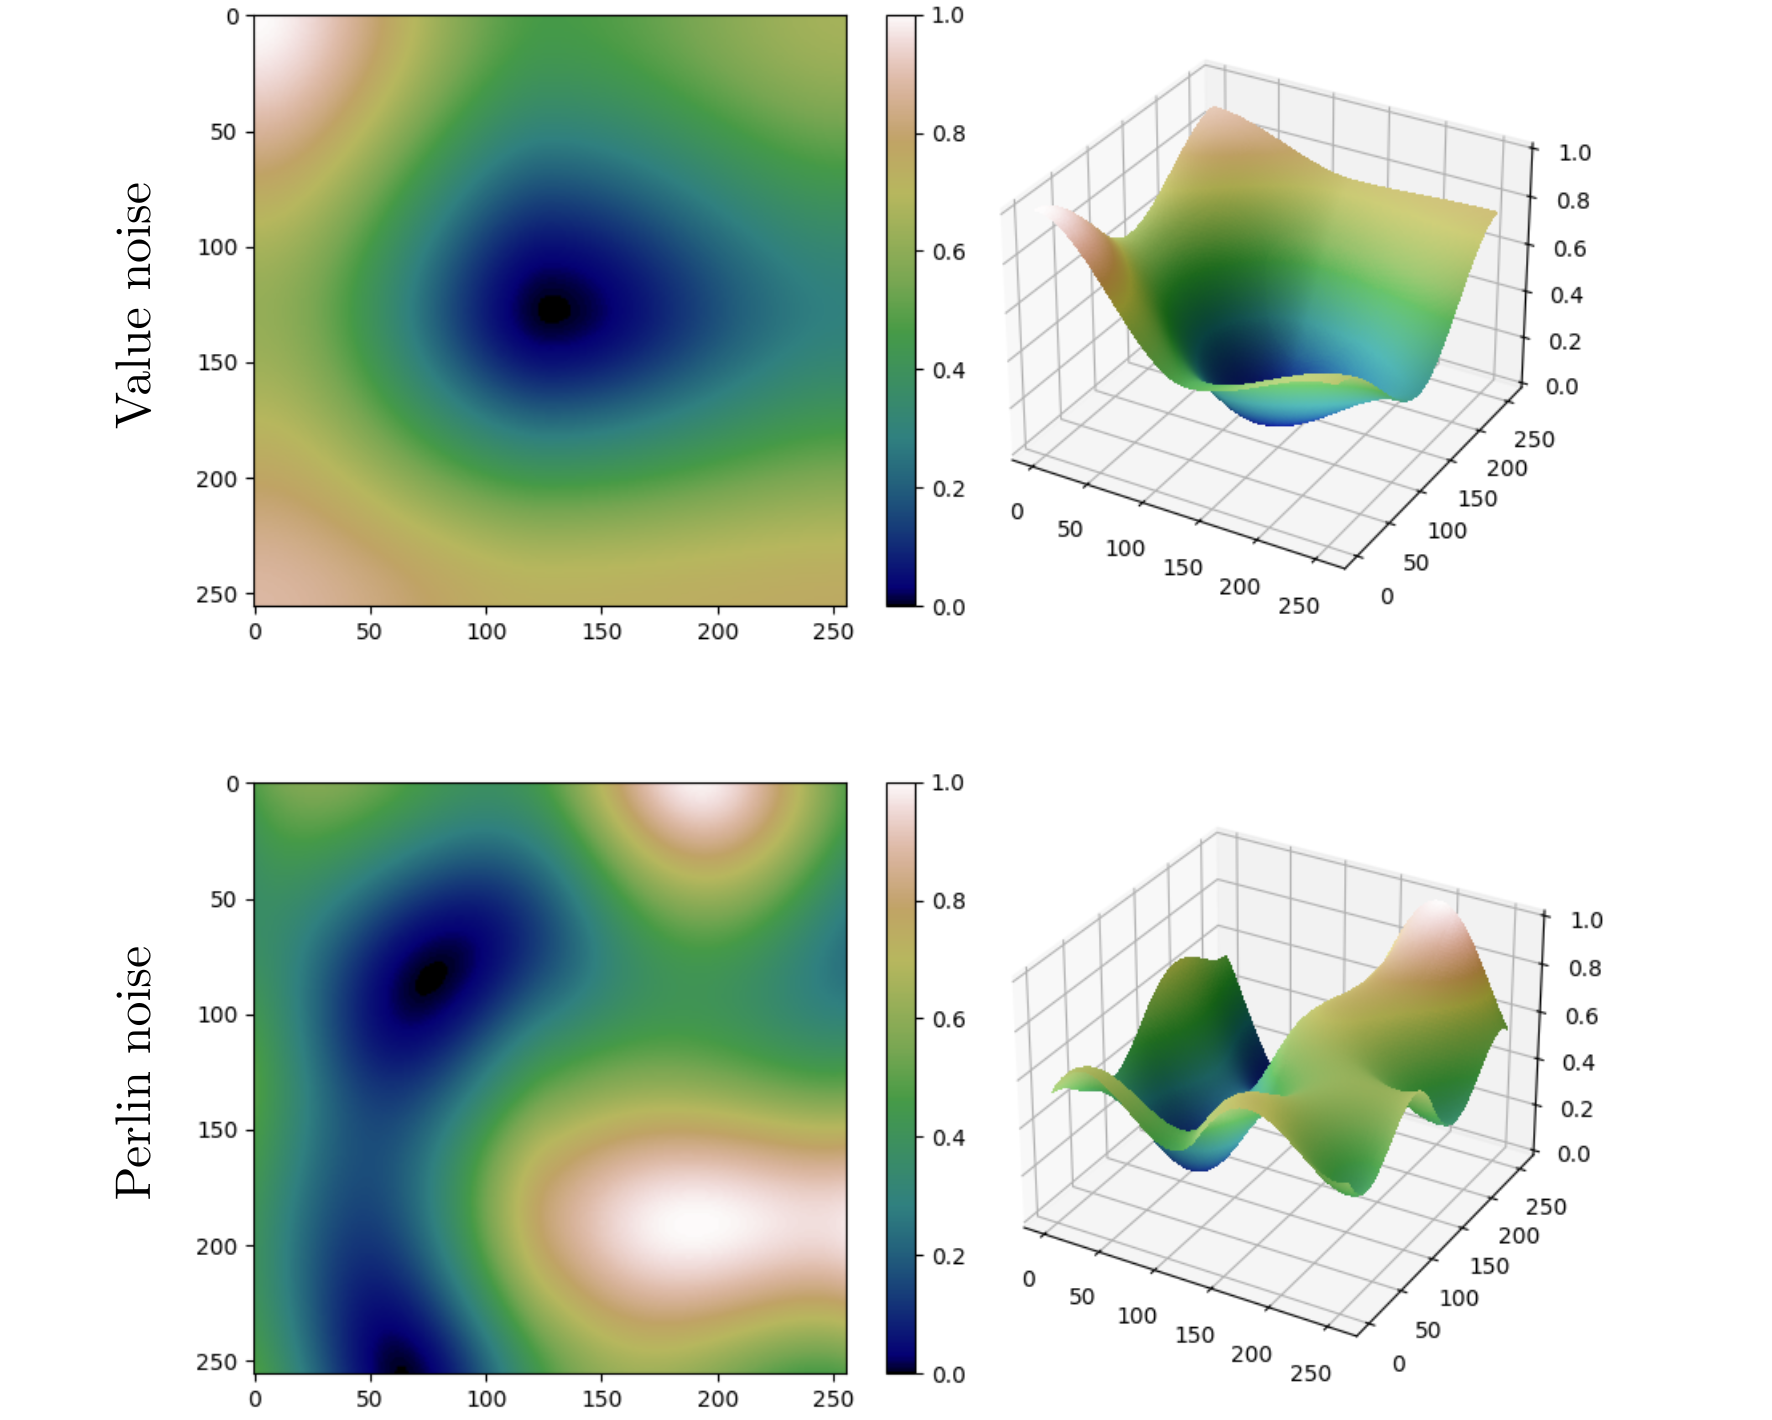
\includegraphics[width=\textwidth]{one layer noise.png}
    \caption{Single-octave Value and Perlin noise}
    \label{fig:single}
\end{figure}

As one may have noticed, since we have yet to add the fractal layers on this base layer, the terrain looks very artificial and unrealistic due to 
the overly smooth appearance. This is because a single-octave noise function lacks the high-frequency details and variation that give natural terrain 
its ruggedness and complexity. By introducing additional octaves through fractal summation, we can simulate the self-similar structure observed in 
real-world landscapes and significantly enhance visual realism. 

After calculating the remaining fractal layers, normalised height values were plottted on a 3D graph, resulting in Figure \ref{fig:plot_vf_pf}. 
\begin{figure}[H]
    \centering
    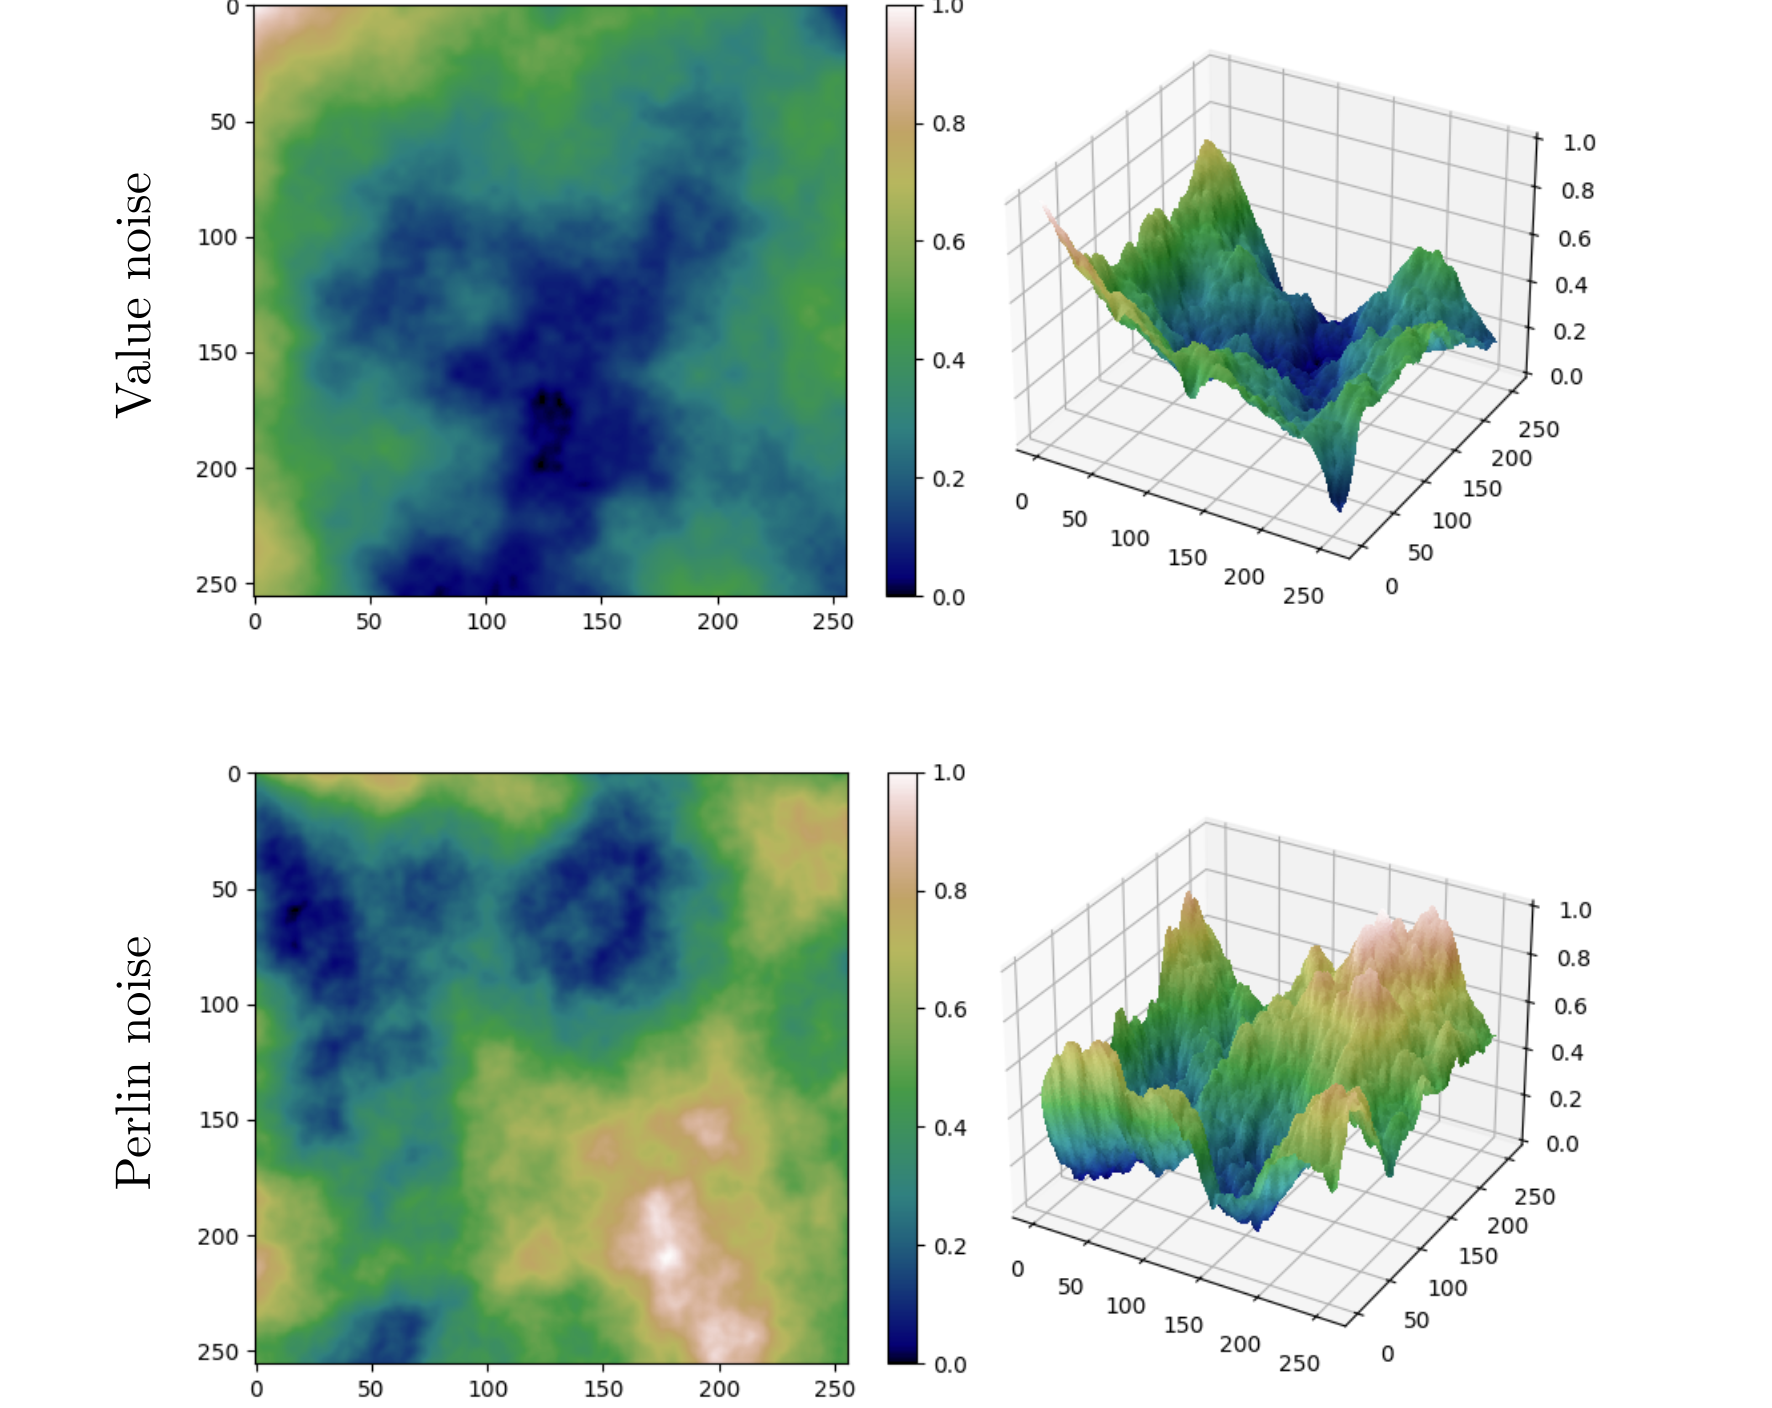
\includegraphics[width=\textwidth]{fractal noises.png}
    \caption{Plots of Value fractal noise and Perlin fractal noise}
    \label{fig:plot_vf_pf}
\end{figure}
We could see that this new terrain greatly enhance the quality of the terrain compared to Figure \ref{fig:single}. This is because each successive layer 
in a fractal noise adds finer detail (achieved through increasing the frequency) to the terrain while preserving the overall structure (by diminishing 
the amplitude of each layer) provided by the first layer. This multi-scale layering captures the hierarchical nature of natural topography, where broad 
mountain ranges coexist with smaller hills and surface irregularities.

After the calculations are completed, I now try to visually compare the Value noise and Perlin noise generated to assess which one produces an overall 
more realistic terrain.

\subsection{\textsc{Visual Comparison}}
\vspace*{-10pt}
The terrain output from Value noise and Perlin noise demonstrates fundamentally different characteristics when generated under identical parameters. 
The value noise terrain exhibits more broad and low-frequency features with fewer pronounced peaks. On the other hand, the Perlin noise terrain reveals 
a more “rugged” topology, characterized by the presence of higher frequency components such as sharper ridges and denser distribution of elevation extrema.  

While value noise is theoretically prone to producing artifacts due to its reliance on scalar interpolation between grid points, such artifacts are not 
prominently visible in the implementation due to the use of high-resolution grids. However, subtle evidence of value's noise limitations is still observable 
in Figure \ref{fig:limitations}, where certain regions appear to exhibit what may be interpreted as artifact-like features. For instance, the region near $(130,170)$ (Artifact 
zone 1, red box) shows an extreme lowland with steep boundaries. Likewise, this type of artifact with sudden changes in elevation can also be spotted near 
$(252,0)$ (Artifact zone 2, orange box). 

\begin{figure}[H]
    \centering
    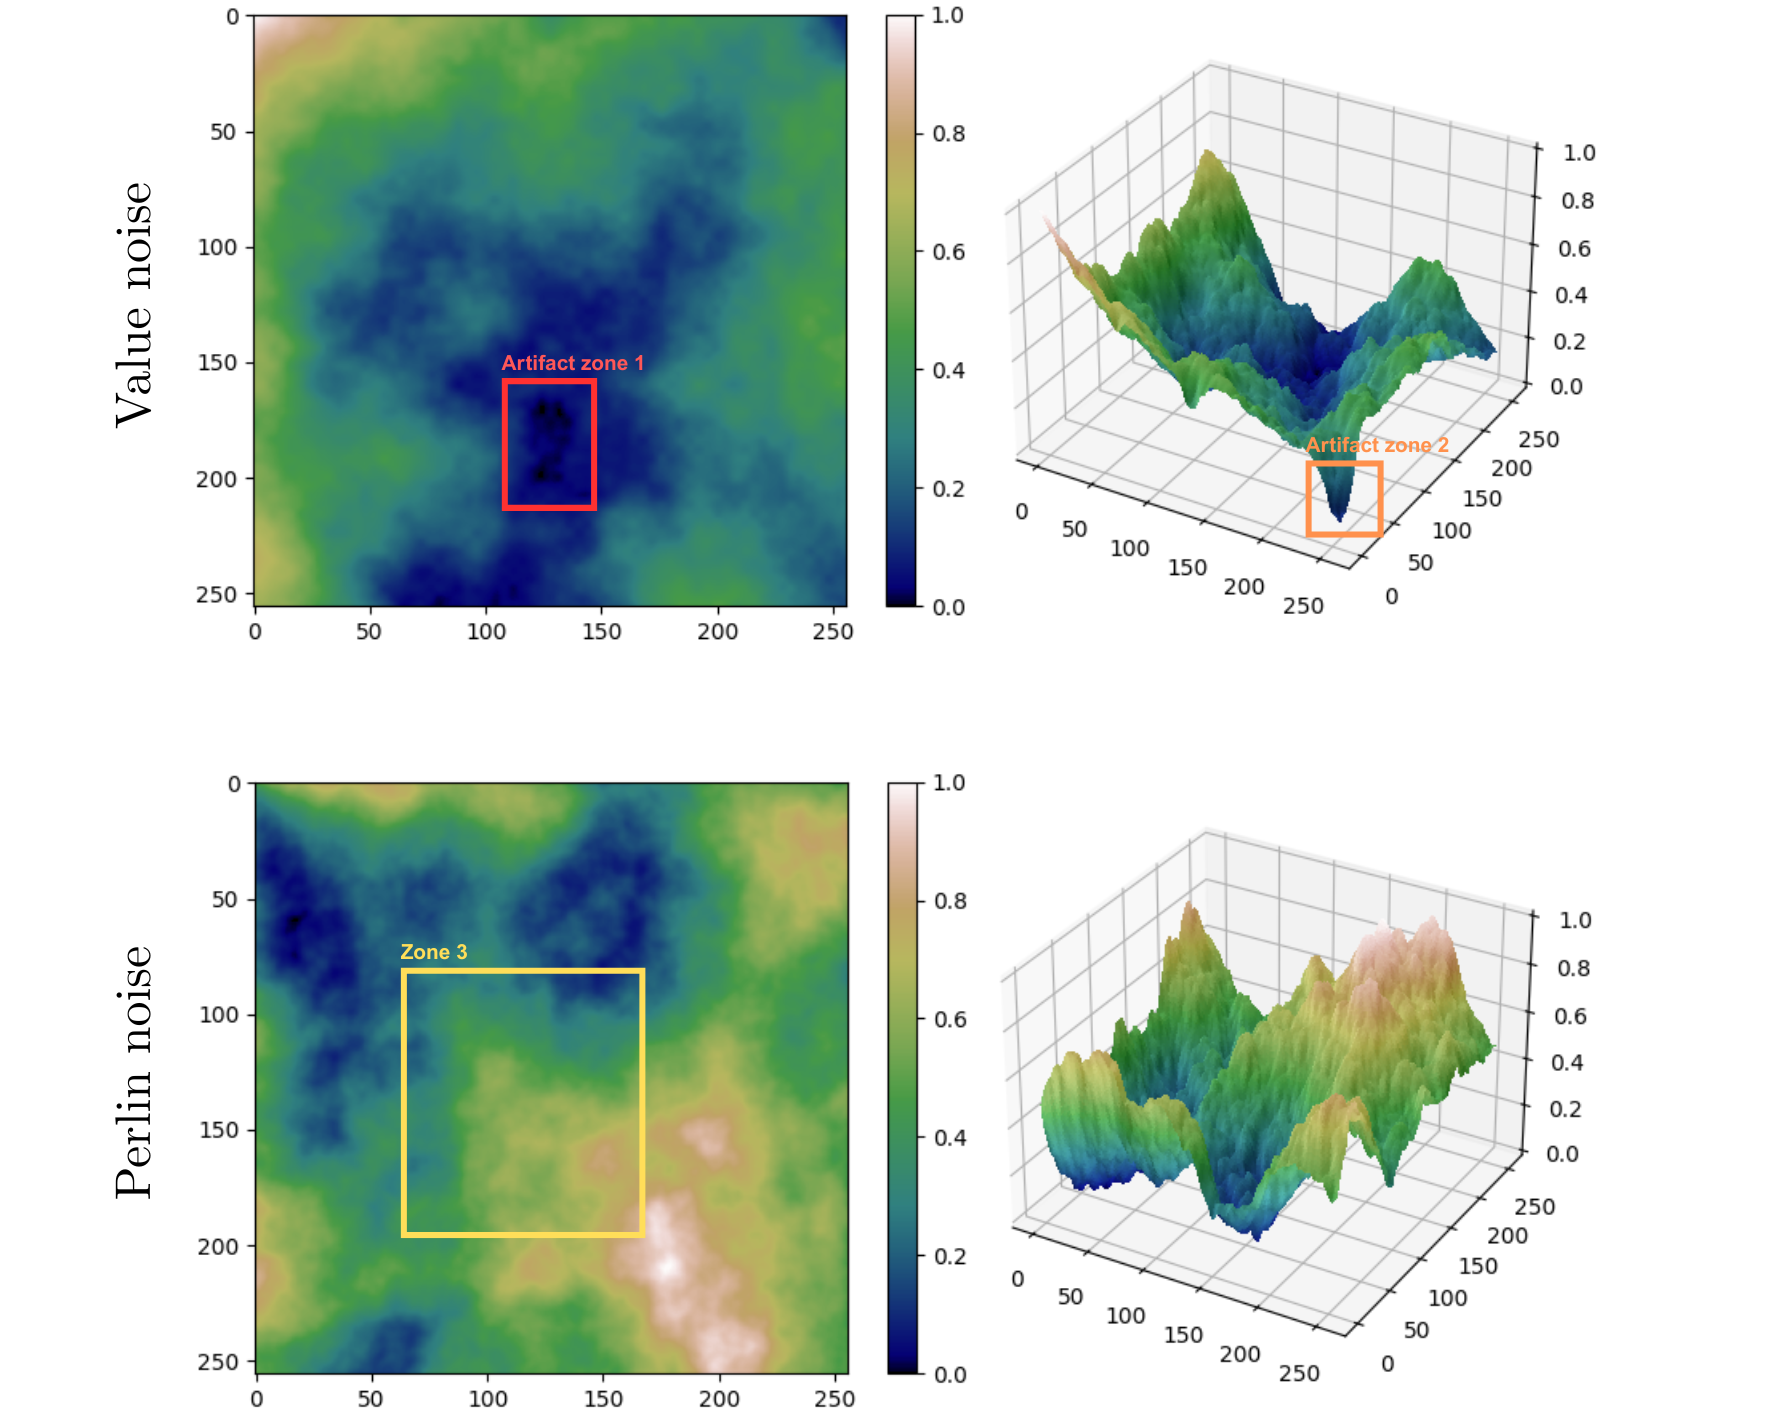
\includegraphics[width=\textwidth]{limitations.png}
    \caption{Visual comparisons, annotated from Figure \ref{fig:plot_vf_pf}, between the two noise types}
    \label{fig:limitations}
\end{figure}

In contrast, the Perlin noise terrain exhibits more continuous and coherent elevation transitions, evidenced by the smoother gradient from peaks to valleys (Zone 3, yellow box). 
This was achieved through gradient-based interpolation, which prevents the formation of artifacts as they are guided by the directional change of the terrain, 
not by flat scalar values. 

However, the distinction in realism is subtle and subjective, and thus these noises should be primarily evaluated with quantitative metrics mentioned in Section \ref{quant_metrics}. 

\subsection{\textsc{Quantitative Comparison}}
\vspace*{-10pt}

For a fair comparison, elevation data from GMTED2010 will first be resampled by taking a weighted average to the same size as the noise function $(256\times256)$, before normalizing 
to the range $[0,1]$. The geographic areas I have selected to compare the noise functions against can be seen in Table \ref{table:first_pick}.

\begin{table}[h!]
    \begin{tblr}{
        colspec={X[1.25,l] X[1.75,l] X[2.75,l] X[3,l]},
        width=\textwidth,
        hlines,
        row{1} = {gray9},
        rowsep=5pt,
    }
        \textbf{Region} & \textbf{Bounding box} & \textbf{Features} & \textbf{Test criteria} \\
        Swiss Alpes & 6.0°E-10.0°E, 45.5°N-47.5°N & pointy peaks and deep valleys & ability to create sharp ridges and smooth valley floors \\
        Himalayan Foothills & 85.0°E-87.0°E, 27.0°N-29.0°N & dense networks of parallel ridges and valleys & ability to produce organized, directional patterns \\
        Rocky Mountains & 7.65°E-7.70°E, 45.98°N-46.02°N & mix of rugged peaks and high flat plains & ability to blend steep slopes with gentle areas
    \end{tblr}
    \caption{Initial pick of geographical regions for quantitative comparisons}
    \label{table:first_pick}
\end{table}
\begin{figure}[H]
    \centering
    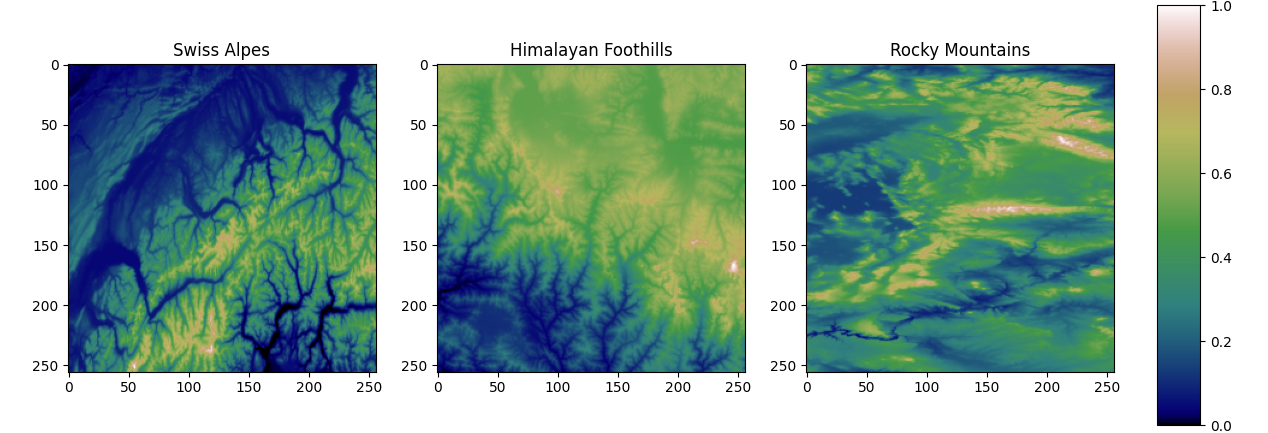
\includegraphics[width=\textwidth]{real data 2d.png}
    \caption{Initial real-life data plot}
    \label{fig:heatplot_realInit}
\end{figure}
The varied real-world terrains will ensure comprehensive evaluation of noise functions' ability to replicate elevation distribution statistics, spatial autocorrelation properties, 
and spectral properties.

However, when these terrains were plotted in Figure \ref{fig:heatplot_realInit}, it became apparent that my original selection of geographic regions needed to be reconsidered. The areas I had chosen spanned 
vast mountain ranges with highly complex and large-scale features. When these were down sampled to fit the $256\times256$ resolution required by my noise implementation, much of the detail 
and variability inherent to the original landscapes was lost. In contrast, my noise-generated terrains, constrained by both resolution and simplicity, tended to produce isolated 
mountainous forms rather than broad, interconnected ranges. Therefore, a new table of chosen geographic regions with scales more closely aligned with the spatial scope of my simulated 
terrains was created (Table \ref{table:final_pick}). 

\begin{table}[h!]
    \begin{tblr}{
        colspec={X[1.25,l] X[1.75,l] X[2.75,l] X[3,l]},
        width=\textwidth,
        hlines,
        row{1} = {gray9},
        rowsep=5pt,
    }
        \textbf{Region} & \textbf{Bounding box} & \textbf{Features} & \textbf{Test criteria} \\
        Everest & 86.9°E-87.0°E, 27.9°N-28.0°N & sharp peaks, deep valleys, extreme elevation gradients & ability to create sharp ridges and smooth valley floors \\
        Denali & 151.0°W-150.5°W, 63.0°N-63.2°N & parallel ridges from glacial flow & ability to produce directional patterns and consistent slope \\
        Matterhorn & 7.65°E-7.70°E, 45.98°N-46.02°N & mix of rugged peaks and gentle terrain & ability to have variations of features
    \end{tblr}
    \caption{Final pick of geographical regions for quantitative comparisons}
    \label{table:final_pick}
\end{table}
\begin{figure}[H]
    \centering
    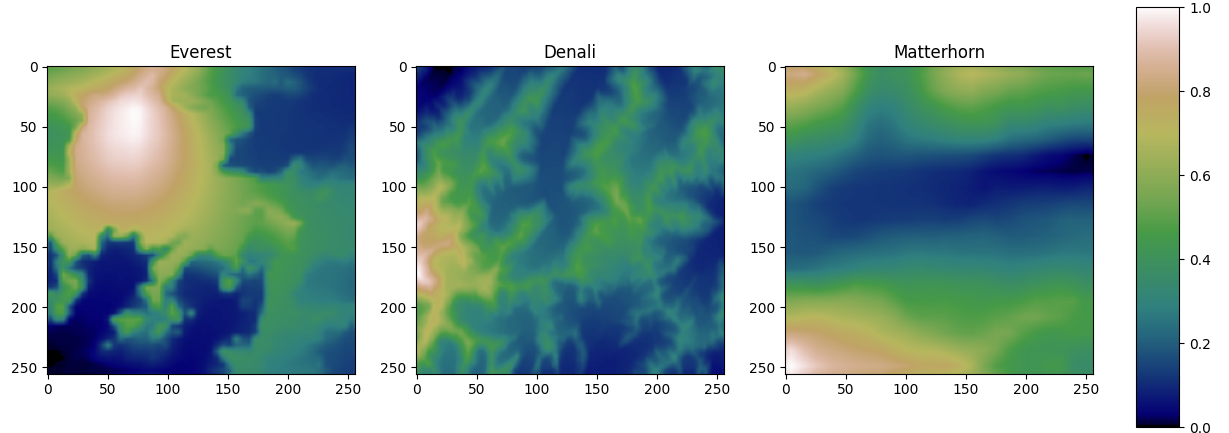
\includegraphics[width=\textwidth]{new real data 2D.png}
    \caption{Re-selected real-life data plot}
    \label{fig:heatplot_realFinal}
\end{figure}
Now that we have selected the terrain, I then use technology to compute the numerical statistical values listed in Section \ref{quant_metrics} for each of the 
real-life data. All of these results, rounded to 4 decimal places, are summarized in Table \ref{table:real_stats}.

\begin{table}[h!]
    \begin{tblr}{
        colspec={X[1,l] X[1,l] X[1,l] X[1,l] X[1,l] X[1,l] X[1,l]},
        width=\textwidth,
        hlines,
        row{1} = {gray9},
        rowsep=5pt,
    }
        \textbf{Region} & \textbf{Mean} & \textbf{Variance} & \textbf{Kurtosis} & \textbf{Skewness} & \textbf{TRI} & \textbf{Moran's I}\\
        Everest & 0.4071 & 0.0770 & -1.0391 & 0.4042 & 0.0086 & 0.9559 \\
        Denali & 0.2963 & 0.0260 & 1.7975 & 1.2217 & 0.0093 & 0.9205 \\
        Matterhorn & 0.3678 & 0.0443 & -0.4070 & 0.5347 & 0.0046 & 0.9833
    \end{tblr}
    \caption{Statistical measures of real-life data}
    \label{table:real_stats}
\end{table}

A histogram was also plotted and is shown here in Figure \ref{fig:histogram_real}
\begin{figure}[H]
    \centering
    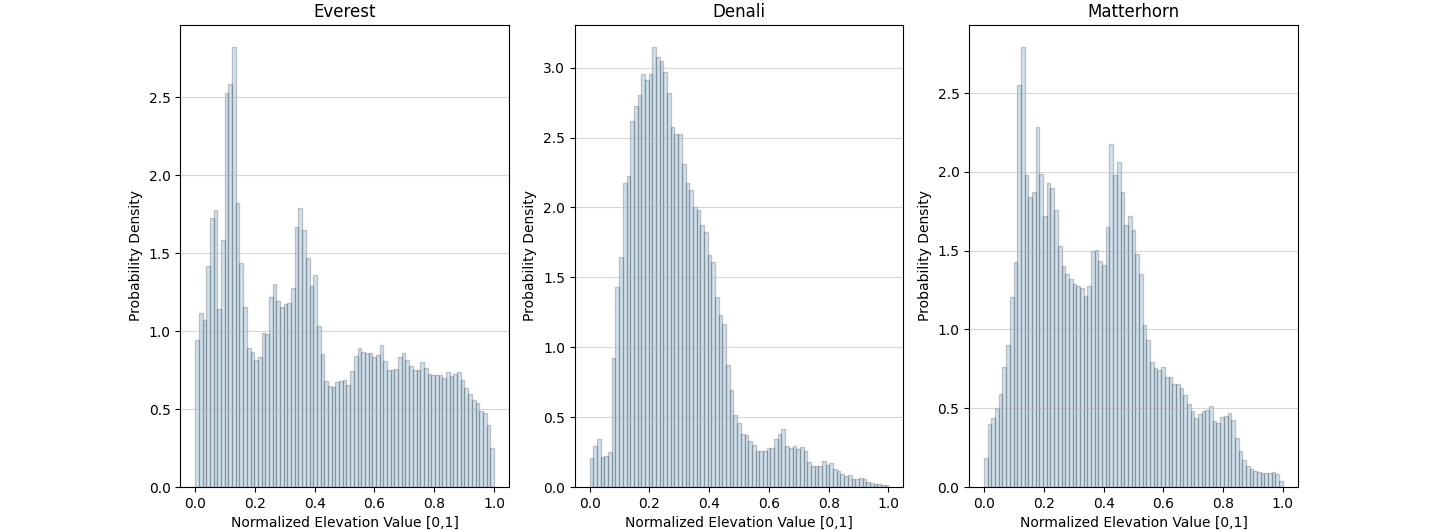
\includegraphics[width=\textwidth]{histogram real life data.png}
    \caption{Reselected real-life probability density histogram}
    \label{fig:histogram_real}
\end{figure}

The mean elevation values obtained aligns with known elevation profiles, with Everest being the highest, followed by Matterhorn and Denali. The variance metric indicates Everest exhibits 
the most heterogeneous elevation distribution, consistent with its complex topography featuring dramatic shifts between high peaks and deep valleys as seen in Figure \ref{fig:heatplot_realFinal}. Denali's notably 
lower variance suggests more uniform elevation changes, while Matterhorn occupies the intermediate position. Kurtosis values reveal fundamentally different distribution shapes: Denali's 
positive kurtosis indicates leptokurtic distribution, suggesting concentrated elevation around the mean with extreme outliers with flatter terrain. In contrast, Everest and Matterhorn 
showed platykurtic distributions, implying more uniform elevation spread. Skewness values are universally positive, showing that all regions have more low-frequency features, though 
Denali's exceptionally high skewness showed disproportionate representation of lower elevations, which reflects its massive base compared to its summit. 

The Terrain Ruggedness Index (TRI) presents an interesting inversion, with Denali showing slightly greater roughness than Everest, despite Everest's higher variance. This suggests 
Denali's elevation changes are more locally concentrated, while Everest's variations are more globally distributed. Matterhorn's notably lower TRI indicates smoother transitions, 
consistent with its relatively uniform appearance in Figure \ref{fig:heatplot_realFinal}. Finally, Moran's I spatial autocorrelation values confirm strong elevation clustering, with Matterhorn exhibiting near-perfect 
spatial dependence. This is evident in that we can all clearly discern clusters of high elevation from clusters of low elevation. 

Next, the PSD of the selected terrains were also computed using technology and is shown in Figure \ref{fig:PSD_real}
\begin{figure}[H]
    \centering
    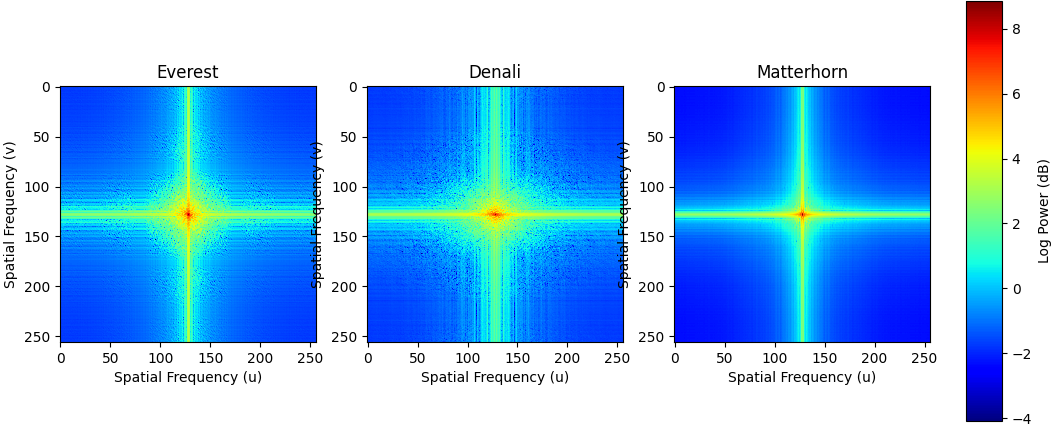
\includegraphics[width=\textwidth]{psd real life.png}
    \caption{PSD of the reselected real-life data}
    \label{fig:PSD_real}
\end{figure}
The PSD clearly corrbates the statistical measures in Table \ref{table:real_stats}. The PSD for Everest exhibits a broader spread of energy into the mid and high-frequency ranges, evident from the more 
diffused transition from red to green/blue. This aligns with Everest's high variance and kurtosis, reinforcing that Everest exhibit complex terrain morphology featuring both large scale 
elevation changes to fine-scale topographic details. For Denali, the PSD has a stronger central concentration of energy and a rapid falloff, signifying the dominance of low-frequency elements. 
This is also supported by the histogram (Figure \ref{fig:histogram_real}), which shows that there is little variation in the elevation data of Denali. Lastly, for Matterhorn, it retains a strong low-frequency core 
but with more pronounced mid-frequency components than Denali. This matches the variance and skewness in elevation distribution.

This quantitative analysis of Everest, Denali, and Matterhorn terrains establishes critical statistical benchmarks that will serve as essential reference points when evaluating noise-generated 
terrain models. The comprehensive statistical profiles reveal distinct yet consistent geomorphological signatures that must be replicated in synthetic terrains to achieve geological plausibility, 
particularly in their elevation distributions, topographic complexity, and spatial organization.

The parameters for the noise we will be using to compare will be the same as those used to generate Figure 5. Firstly, before comparing it to real-life elevation, I wanted to quantitively 
distinguish Perlin noise and Value noise. Like before, a table of statistical measures were calculated (Table \ref{table:noise_stats}), along with a histogram and the PSD. 

The synthetic elevation models generated using Value noise and Perlin noise display distinct statistical and spatial characteristics. Perlin noise exhibits a higher mean elevation and nearly double 
the variance compared to Value noise, indicating greater vertical heterogeneity and a broader distribution of elevation values. This aligns with the smoother yet more structured gradients typically 
associated with Perlin noise. The increased variance suggests that Perlin terrain incorporates more differentiated features, resembling the unevenness found in natural landscapes. In contrast, the 
lower variance in the Value noise terrain reflects a more homogenous surface with minimal variation in elevation.

\begin{table}[h]
    \begin{tblr}{
        colspec={X[1,l] X[1,l] X[1,l] X[1,l] X[1,l] X[1,l] X[1,l]},
        width=\textwidth,
        hlines,
        row{1} = {gray9},
        rowsep=5pt,
    }
        \textbf{Region} & \textbf{Mean} & \textbf{Variance} & \textbf{Kurtosis} & \textbf{Skewness} & \textbf{TRI} & \textbf{Moran's I}\\
        Value & 0.3041 & 0.0259 & 0.5373 & 0.6560 & 0.0065 & 0.9592 \\
        Perlin & 0.4542 & 0.0454 & -0.8280 & 0.1166 & 0.0101 & 0.9543
    \end{tblr}
    \caption{Statistical measures of noise-generated terrains}
    \label{table:noise_stats}
\end{table}

Kurtosis and skewness values further differentiate the two. The basic Value noise model yields a positive kurtosis, indicating a leptokurtic distribution with a sharper peak around the mean and 
more frequent extreme values. Perlin, by contrast, is distinctly platykurtic, suggesting a flatter distribution with fewer outliers and a more even spread of elevation values. This pattern is 
reinforced by skewness metrics: Value noise shows a strong positive skew, meaning lower elevation values dominate the distribution. Perlin's skewness is closer to zero, indicating a more symmetric 
terrain profile with less pronounced elevation bias.

The Terrain Ruggedness Index (TRI) again favors Perlin, although more subtly, with a slightly higher value compared to Value noise. While both values remain low relative to natural terrains, this 
suggests Perlin includes more local elevation changes and minor features that contribute to a more textured surface. Interestingly, Moran's I values remain high for both, indicating strong spatial 
autocorrelation. While this might be expected for Perlin due to its smooth gradients, the similarly high value for Value noise implies that even random scalar values with no directionality exhibits spatial dependence, 
perhaps due to interpolation during generation.

Yet, when compared to the elevation profiles of real-world landscapes, both synthetic models exhibit a lack of realism. Starting with mean elevation, their modest averages reflect the absence of 
geological processes that typically generate both consistent patterns and extreme variations. Perlin noise, with its higher mean and smoother gradients, shows a weak resemblance to the balanced 
elevation profile of the Matterhorn. In contrast, Value noise, with its lower mean and more irregular characteristics, lacks similarity to any natural elevation structure.

In terms of variance, both models display a limited range, falling short of the broad elevation variability observed in real terrains. Even the Matterhorn, the least variable among the real-world 
examples, exhibits an order-of-magnitude greater heterogeneity. This suggests that neither synthetic model adequately captures the scale of variation resulting from processes such as tectonic 
uplift, erosion, or glacial carving. Although Perlin noise demonstrates a higher variance than Value noise, its fluctuations remain relatively subdued and fail to replicate the spatial intensity 
of natural landscapes.

Regarding kurtosis, Value noise presents a positive value that initially appears similar to Denali's. However, closer examination reveals that this similarity is likely superficial and the result 
of modeling artifacts. Perlin noise, on the other hand, exhibits negative kurtosis, showing a weak alignment with the profiles of Everest and the Matterhorn. Nevertheless, it still lacks the dynamic 
range and feature clustering, such as ridgelines, found in real terrain.

When skewness is considered, Value noise outperforms Perlin noise by favoring low-frequency elevation features. While this statistical resemblance may seem promising, it is important to note that 
natural skewness arises from geomorphological asymmetries not replicated in either model. As a result, the observed skewness in Value noise likely stems from randomness rather than an underlying 
structural basis.

Turning to the Terrain Ruggedness Index (TRI), both synthetic models produce values comparable to those of real-world terrains, indicating a degree of success in capturing fine-scale surface complexity. 
Furthermore, the Moran's I values of both noise types closely align with those of natural landscapes, suggesting that artificial noise functions are capable of mimicking spatial autocorrelation patterns 
found in nature.

\begin{figure}[H]
    \centering
    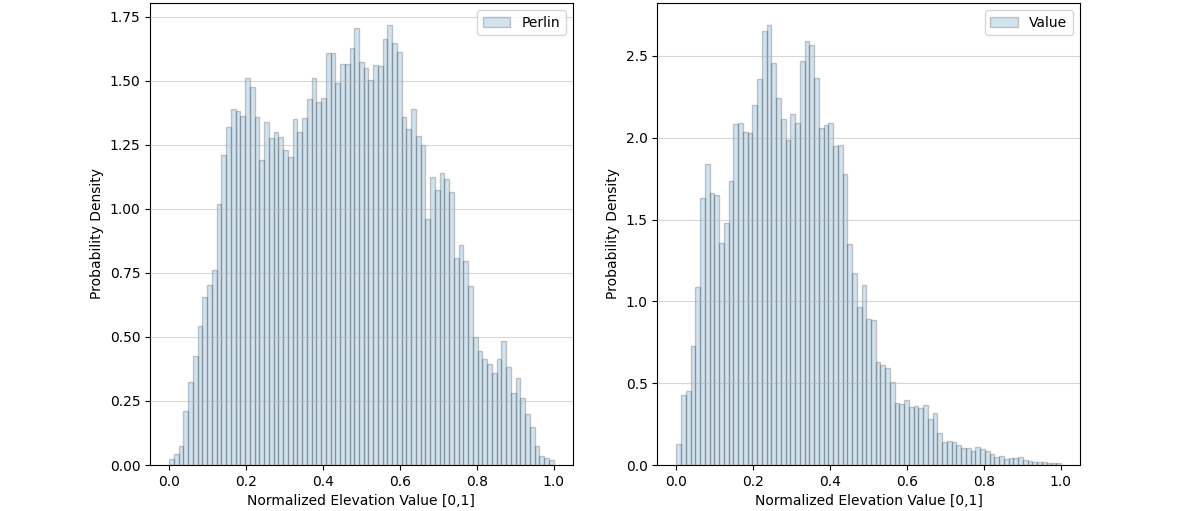
\includegraphics[width=\textwidth]{noise histogram.png}
    \caption{Noise terrain probability density diagram}
    \label{fig:histogram_noise}
\end{figure}

As illustrated in Figure \ref{fig:histogram_noise}, the probability density histogram indicates that Value noise more closely mirrors the elevation distribution observed in real terrains. However, histograms do not account for 
spatial arrangement or topographic continuity. Thus, while Value noise may approximate the statistical distribution of elevations, it still fails to replicate the structural coherence inherent to natural 
landscapes.

\begin{figure}[H]
    \centering
    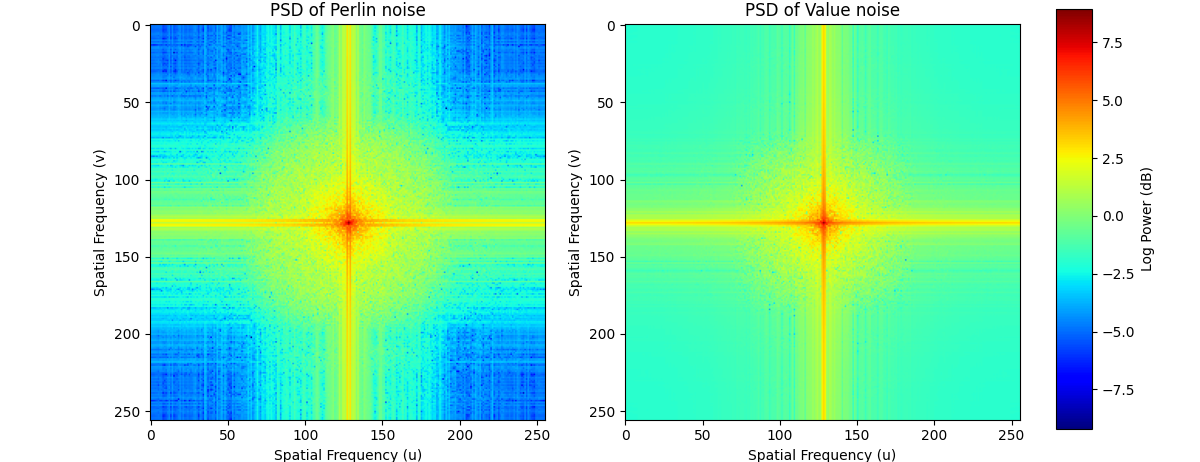
\includegraphics[width=\textwidth]{PSD noise.png}
    \caption{PSD of noise terrains}
    \label{fig:PSD_noise}
\end{figure}

Finally, as seen in Figure \ref{fig:PSD_noise}, The PSD of Perlin noise exhibits a pronounced concentration of energy at low spatial frequencies, visible as a bright central region that smoothly transitions into lower 
power at higher frequencies. This structure loosely resembles the PSDs of the real terrains, particularly Everest and Denali, which also display a central intensity peak with a radial decay, indicating 
a predominance of large-scale terrain features and a tapering of finer details. However, Perlin noise lacks the irregular frequency components evident in real terrains. Real landscapes such as Denali and 
Everest exhibit uneven, speckled distributions in the outer frequency bands, reflecting the complex, non-repeating, and multi-scale nature of geological formations. In contrast, Perlin noise displays a 
more symmetrical decay, characteristic of its algorithmic smoothness and periodicity.

On the other hand, the PSD of Value noise shows a far more uniform and flattened distribution compared to both Perlin noise and natural terrain. The concentration of power around the origin is less intense, 
and the surrounding frequency space remains relatively homogeneous, almost like white noise. Consequently, the Value noise PSD diverges considerably from the real terrain PSDs, where energy-rich low 
frequencies dominate. 


\raggedright
\section{\textsc{Evaluation}}
\hrule height 0.5pt
\vspace*{2.5pt}

While the outcome of this investigation was rather successful, there were notable assumptions and methodological limitations that could 
have been better addressed and improved.

One of the most significant setbacks was the initial decision to generate terrain maps at a resolution $1024\times1042$ pixels. While the intention 
was to match the granularity of real-world terrain, this approach quickly proved computationally efficient, especially for the Moran's I calculations 
which took at least 2 hours to finish for one map. To ensure feasibility within the timeline, I had to reduce the resolution to $256\times256$. Although 
this allowed for smoother experimentation, it introduced the trade off that the lower resolution may not have captured finer-scale topographic features, 
potentially limiting the fairness of direct comparisons with real-world datasets. Even when I tried to resample real-world datasets to match the $256\times256$
resolution of the noise maps, it smoothed and altered the fine-scale features in the original terrain data, which downgraded the accuracy of spatial and 
spectral comparisons. In future investigations, a multiscale analysis could be adopted to examine noise performance at multiple resolutions.  

Moreover, several assumptions were made without rigorous justification. For instance, while constructing the smoothstep functions used in interpolation, I assumed 
that the order must be odd to satisfy a symmetry condition. Although this assumption aligns with some sources, I was unable to produce a formal mathematical proof. 
This is an area where greater rigor could be applied in future iterations of this investigation. 

A similar limitation concern the preference of Moran's I over Geary's C in evaluating spatial autocorrelation. While I justified this based on the focus of my 
analysis on global similarity patterns, I did not conduct a comparative analysis of the two metrics, nor did I examine cases where Geary's C might yield extra 
helpful insights. Including such a comparison could have added depth to my conclusions and strengthened the reliability of the findings. 

Another methodological refinement that could enhance the evaluation of realism is the classification of noise colour. Terrain surfaces, like many natural phenomena, 
often exhibit red noise characteristics, where lower spatial frequencies dominate. Incorporating spectral slope analysis to determine whether the noise resembles 
red, pink, white, or blue noise would offer an additional dimension of realism assessment. Since human perception tends to associate “naturalness” with red noise 
(Haroz, 2006), this framework could help formalize qualitative judgments of visual realism.

I had also utilized only one set of parameters to perform the comparison, which discards numerous other possibilities that could have enhanced the synthetic noise 
similarities to real terrain. This was done because otherwise it would go beyond the scope of this IA. However, in the future, I would investigate with different 
parametric settings; although I cannot include all in the paper, at least I could compile into a concise table and put in the Appendix. 

Finally, a limitation inherent in my methodology was the reliance on a fixed seed for initial comparisons. Larger sample size could have been employed to more 
robustly quantify the variance and confidence in the conclusion. 


\raggedright
\section{\textsc{Conclusion}}
\hrule height 0.5pt
\vspace*{2.5pt}

In conclusion, I successfully achieved my aim of the investigation and demonstrated the superiority of the Perlin noise function in 
simulating realistic terrain features. This was accomplished through a comprehensive evaluation based on both statistical measures, such 
as the Moran's I spatial autocorrelation, and spectral characteristics.

In terms of basic elevation statistics, Perlin noise exhibits a higher mean elevation and greater variance than Value noise. These metrics 
align more closely with natural landscapes, suggesting that Perlin noise better captures the moderate elevation shifts observed in alpine 
topography. Its negative kurtosis further mirrors that of real terrains like Everest and Matterhorn, indicating a flatter distribution with 
fewer extreme outliers. Although Value noise shows a favorable skewness profile, this similarity appears to be an artifact of randomness.

The power spectral density (PSD) analysis provides further evidence in favor of Perlin noise. Its frequency domain representation reveals 
a strong central energy concentration and a gradual decay towards higher frequencies, resembling the spectral patterns observed in terrains 
such as Everest and Denali. In contrast, Value noise produces a flatter, more uniform PSD. The absence of distinct low-frequency dominance 
and directional variation implies a lack of structural realism.

However, both synthetic models remain fundamentally limited in capturing the true complexity of real-world landscapes. Not only did both 
fail to capture the full statistical range observed in natural terrain, most notably the variance metric, its PSD stray far from resembling 
the frequency decay observed in natural terrain. 

This inquiry has significantly deepened my understanding of noise functions, particularly how their underlying mathematical foundations 
and algorithms influence their capacity to replicate the complexity and variability found in natural landscapes. Additionally, the research 
process broadened my knowledge with statistical tools and introduced me to spectral analysis and signal processing techniques, most notably 
the use of Power Spectral Density, which I had not encountered before.

Given that this area of study remains relatively underexplored, with limited literature due to the high competition between game companies, 
I often found myself navigating through a labyrinth with few established guidelines. While this was challenging, the lack of precedent also 
gave me the freedom to formulate and test original approaches. I am particularly proud of the fact that many of the techniques and comparisons 
I employed were conceptualized on my own. This experience serves more than just a stepping-stone for my problem-solving and analytical abilities 
but also affirmed my enthusiasm for mathematical research. 

Looking ahead, I am eager to further explore this topic at the university level, where I can apply more advanced and rigorous mathematical tools 
and contribute to a promising field with fresh insights and greater technical depth.  


\appendix

\end{document}